\documentclass[12pt]{article}
\usepackage[top=1in, bottom=1in, left=1in, right=1in]{geometry}

\usepackage{setspace}
\onehalfspacing

\usepackage{amssymb}
%% The amsthm package provides extended theorem environments
\usepackage{amsthm}
\usepackage{epsfig}
\usepackage{times}
\renewcommand{\ttdefault}{cmtt}
\usepackage{amsmath}
\usepackage{graphicx} % for graphics files

% Draw figures yourself
\usepackage{tikz} 

% writing elements
\usepackage{mhchem}

% The float package HAS to load before hyperref
\usepackage{float} % for psuedocode formatting
\usepackage{xspace}

% from Denovo Methods Manual
\usepackage{mathrsfs}
\usepackage[mathcal]{euscript}
\usepackage{color}
\usepackage{array}

\usepackage[pdftex]{hyperref}
\usepackage[parfill]{parskip}

% math syntax
\newcommand{\nth}{n\ensuremath{^{\text{th}}} }
\newcommand{\ve}[1]{\ensuremath{\mathbf{#1}}}
\newcommand{\Macro}{\ensuremath{\Sigma}}
\newcommand{\rvec}{\ensuremath{\vec{r}}}
\newcommand{\vecr}{\ensuremath{\vec{r}}}
\newcommand{\omvec}{\ensuremath{\hat{\Omega}}}
\newcommand{\vOmega}{\ensuremath{\hat{\Omega}}}
\newcommand{\sigs}{\ensuremath{\Sigma_s(\rvec,E'\rightarrow E,\omvec'\rightarrow\omvec)}}
\newcommand{\el}{\ensuremath{\ell}}
\newcommand{\sigso}{\ensuremath{\Sigma_{s,0}}}
\newcommand{\sigsi}{\ensuremath{\Sigma_{s,1}}}
%---------------------------------------------------------------------------
%---------------------------------------------------------------------------
\begin{document}
\begin{center}
{\bf NE 250, F15\\
September 30, 2015 
}
\end{center}

Announcements:
\begin{itemize}
\item How I grade paragraphs
\item homework due friday; I'll also assign the next one that day
\end{itemize}

---------------------------------\\
\underline{Criticality and Eigenproblems}
\begin{itemize}
\item Criticality refers to a self-sustaining \textit{and} controlled chain reaction $\rightarrow$ production = losses
\item subcritical: production $<$ loss $\rightarrow$ chain reaction cannot sustain itself
\item supercritical: production $>$ loss $\rightarrow$ chain reaction increases 
\end{itemize}
%
In the transport model (separation of variables):
\[\psi(\rvec, E, \vOmega, t) = T(t) \Psi(\rvec, E, \vOmega) \:.\]
Plug this in and divide by $\psi$ to get
\[\frac{1}{T}\frac{dT}{dt} = \frac{v}{\Psi} L \Psi(\rvec, E, \vOmega) = \alpha \:.\]
%
Here, $L$ contains streaming, total, scattering, and fission operators.

Because the TE is linear, we can use the principle of superposition. 
therefore, the general solution is the sum of \textbf{all} permissible solutions indicated by $\alpha$.

This means time dependence looks like
\[ T(t) = \tau \exp(\alpha t)\]
where $\tau$ is a constant of integration determined by the initial condition.
Then
\[L\Psi = \frac{\alpha}{v}\Psi\]
%
We assume (which is usually true) that the boundary conditions are homogeneous (that is, have no fixed parts).
In this case, we have a linear and homogeneous system.

$\Psi(\rvec, E, \vOmega) = 0$ is a valid solution, but it is the trivial one.

``Eigenvalues" are special values of $\alpha$ for which non-trivial solutions are valid.
for example
\begin{align*}
(L - \frac{\alpha}{v})\Psi &= 0 \:, \quad \in \mathbb{R} \\
\Psi \neq 0 \rightarrow \: &\alpha = v L
\end{align*}
%
The solutions for this problem are eigenfunctions determined to within a multiplicative constant.
If you fine a $\Psi$ that is a solution, then $c \Psi$ is also a solution, where $c$ is a constant:
\[L(c \Psi) = cL \Psi = \frac{\alpha}{v}c \Psi \:.\]

Thus, we want to solve the Eigenproblem: $L\Psi(\rvec, E, \vOmega) = \frac{\alpha}{v}\Psi(\rvec, E, \vOmega)$.\\
A non-trivial solution requires $(L - \frac{\alpha}{v})$ is singular. \\
That is, for $\Psi \neq 0 \rightarrow \: \alpha = v L$, which causes $L - \frac{\alpha}{v}$ to be zero, or non-invertible.


----- aside ----\\
Linear operators: $L(a*x + b*y) = aL(x) + bL(y)$, where $a$ and $b$ and constants and $x$ and $y \: \in \: L$.\\
Examples are the derivative operator and integration. \\
A counter example is a quadratic:
\begin{align*}
L(z) &= z^2 \\
L(a(x) + b(y)) &= (ax + by)^2 = a^2 x^2 + axby + b^2 y^2 \\
& \neq \underbrace{a x^2}_{aL(x)} + \underbrace{b x^2}_{bL(x)}
\end{align*}
-------\\
Our transport operator is linear, so each eval gives an emode, and the solution is a superposition of all emodes. \\
The collection of evals defines the spectrum of $L$.

Superposition of emodes for the general soln of the TE:
\begin{align*}
\psi(\rvec, E, \vOmega, t) &= \sum_{j} \tau_j \exp[\alpha_j t] \Psi_j(\rvec, E, \vOmega) \\
\psi(\rvec, E, \vOmega, 0) &= \sum_{j} \tau_j \Psi_j(\rvec, E, \vOmega) \quad \text{(known)}
\end{align*}

The fundamental emode corrsponds to $\max(Re(\alpha_j))$
\begin{itemize}
\item critical: $\max(Re(\alpha_j)) = 0$ for some $j$. All components but this one will attenuate. 
\item subcritical: $\max(Re(\alpha_j)) < 0 \: \forall j$.
\item supercritical: $\max(Re(\alpha_j)) > 0$ for some $j$, which gives growing eigenmode(s).
\end{itemize}
We denote the fundamental mode by $j=0$, $\alpha_0$. \\
This dominates the solution as $t \rightarrow \infty$:
\[\lim\limits_{t \to \infty} \psi(\rvec, E, \vOmega, t) = \Psi_0(\rvec, E, \vOmega)\]
and $\Psi_0$ must be real and positive.

\begin{itemize}
\item $\alpha_0 = 0$ is the criticality condition; gives a singular operator.
\item \textit{Given} a composition and geometry, $\alpha_j \rightarrow \psi$ for all time.
\item \textit{Determine} composition and geometry, $\alpha_0 = 0$ for criticality, $\alpha_j$ are evals.
\end{itemize}

%------------------------------------------------------------
\vspace*{1 em}
\underline{Existence of SS Soln to TE}
\[\frac{1}{v}\frac{\partial \psi}{\partial t} = L\psi + S = 0\]
in steady state (assumes $L$ and $S$ are time independent).

\begin{enumerate}
\item $\alpha_0 < 0$: $\psi$ decays in time; there is a non-zero $\psi$ that balances production and loss $\rightarrow$ a ss soln exists.
\item $\alpha_0 = 0$: if $S \neq 0$, then ss soln is unbounded \\
\hspace*{3.5 em}if $S=0$, then ss soln is $\Psi_0$.
\item $\alpha_0 > 0$: a bounded ss soln does \textit{not} exist unless $S=0$ and $\Psi_0 = 0$.
\end{enumerate}

%------------------------------------------------------------
\vspace*{1 em}
\underline{Effective multiplication factor}\\
All of that is a bit restrictive. 
Instead, we can use a mathematical shift to give us more flexibility. 

Alter the effective fission yield, $\nu$, by scaling it with $k$. 
This allows us to vary $k$ to achieve $\alpha_o = 0$.
%
\begin{align*}
\vOmega \cdot \nabla \psi(\vec{r}, E, \vOmega) &+ \Sigma_t \psi(\vec{r}, E, \vOmega) = \int_{4 \pi} d\vOmega' \int_0^{\infty} dE' \: \Sigma_s(E', \vOmega' \rightarrow E, \vOmega) \psi(\vec{r}, E', \vOmega')\\
 +& \underbrace{\frac{1}{k}}_{\text{new}}\frac{\chi(E)}{4 \pi}\int_0^{\infty} dE' \: \nu(E') \Sigma_f(E') \int_{4 \pi} d\vOmega' \:\psi(\vec{r}, E', \vOmega')
\end{align*}
%
+ homogeneous boundary conditions.
\begin{itemize}
\item $k$ as a multiplication factor: the ratio of neutron production in one generation to the neutron production in the previous generation.
\item Let's define $p$ as all phase space, then
  \[\int dp = \int_{V} d\rvec \int_{4 \pi} d\vOmega \int_0^{\infty} dE\]
\item compute neutron production in $p$:
  \[\int dp\:\frac{\chi(E)}{4 \pi}\int_0^{\infty} dE' \: \nu(E') \Sigma_f(E') \int_{4 \pi} d\vOmega' \:\psi(\vec{r}, E', \vOmega') \]
\item compute neutron losses in $p$:
  \[\int dp\:\biggl[\vOmega \cdot \nabla \psi + \Sigma_t \psi - \int_{4 \pi} d\vOmega' \int_0^{\infty} dE' \: \Sigma_s(E', \vOmega' \rightarrow E, \vOmega) \psi(\vec{r}, E', \vOmega') \biggr] \]
\item ss: losses in this generation = production in the immediate past generation.
\item $k$ is the ratio of these two equations, giving the multiplication factor over $p$.
\item Note that $p$ is arbitrary, it applies pointwise over the system (limit as $V$ goes to zero).
\item $k=1$ corresponds to criticality.
\end{itemize}

We can compare this formulation (which we're more used to) to the $\alpha$ version, which is used more frequently at LLNL and LANL, for example.
%
\begin{align*}
\vOmega \cdot \nabla \psi &+ \bigl(\Sigma_t + \underbrace{\frac{\alpha_0}{v}}_{\text{new}}\bigr)\psi = \int_{4 \pi} d\vOmega' \int_0^{\infty} dE' \: \Sigma_s(E', \vOmega' \rightarrow E, \vOmega) \psi(\vec{r}, E', \vOmega')\\
 +& \frac{\chi(E)}{4 \pi}\int_0^{\infty} dE' \: \nu(E') \Sigma_f(E') \int_{4 \pi} d\vOmega' \:\psi(\vec{r}, E', \vOmega')
\end{align*}
%
\begin{itemize}
\item we can see that $k=1$ means $\alpha_0 = 0$ and vice versa.
\item $\alpha$-eval problem: the total xsec is modified by a 1/v absorber.
\item There is numerical difficulty if $\alpha_0 < 0$.\\
If $\frac{-\alpha_0}{v} > \Sigma_t$ then total interaction becomes a ``source" rather than a loss!
\item If $\alpha_0 > 0$, absorption of \textbf{slow} neutrons is enhanced by a $\alpha_0$/v absorber $\rightarrow$ harder spectrum.
\item If $\alpha_0 < 0$, absorption of \textbf{fast} neutrons is enhanced by a $\alpha_0$/v absorber $\rightarrow$ softer spectrum.
\item This is important b/c rxn rate is $\int_0^{\infty} dE \Sigma_j(E) \phi(E)$
\end{itemize}


%------------------------------------------------------------
\vspace*{1 em}
\underline{Integral form of TE} using MOC formalism (B\&G 1.2).\\
The neutron transport equation is an integro-differential equation for the
neutron angular density (or flux). We will derive an equivalent integral equation. This raises the question of whether there is or is not also an
equivalent purely differential expression for the neutron transport problem.
The answer is that there is not. In deriving the transport
equation it was necessary to consider the neutron angular density in the 
immediate (space-time) vicinity only of the point under consideration, whereas the
whole range of energies and angles had to be included in the transport equation
for the angular density at a particular energy and angle. Hence, the formulation
IS local, involving derivatives, in space and time, but it is extended, involving
integrals, in energy and angle.

In a collision, the position
and time associated with a neutron change continuously whereas the energy and
angle will change in a discontinuous manner. As a consequence, a mathematical
formulation of the neutron transport problem must contain integrals over energy
and angle.

Since the neutron transport equation is a linear first order partial differential-
integral equation, it can be converted into an integral equation by a standard
procedure known as the \textit{method of characteristics}.

\[\vOmega \cdot \nabla \psi(\rvec, \vOmega, E) + \Sigma_t \psi(\rvec, \vOmega, E) = q(\rvec, \vOmega, E)\:,\]
where $q$ contains fixed, inscattering, and fission sources. \\

\begin{figure}[h!] 
    \label{fig:cosines}
    \begin{center}
    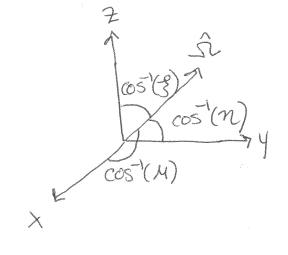
\includegraphics[keepaspectratio, width = 2 in]{../figs/cosines}
    \end{center}    
\end{figure}
%
The streaming term is 
\begin{align*}
\vOmega \cdot \nabla \psi(\rvec, \vOmega, E) &= \mu \frac{\partial \psi}{\partial x} + \eta \frac{\partial \psi}{\partial x} + \xi \frac{\partial \psi}{\partial z} \\
\mu^2 &+ \eta^2 + \xi^2 = 1 \\
\vOmega &= \mu \hat{x} + \eta \hat{y} + \xi \hat{z}
\end{align*}
%
Note that in this figure $\vOmega$ is a direction of motion of a point on a unit sphere, not a point in space.

We will use the figure below in our derivation with $\vec{r} = \rvec_0 + s(\mu \hat{x} + \eta \hat{y} + \xi \hat{z})$, where $\rvec_0$ is an arbitrary point.
Further $x = x_0 + s\mu$, $y = y_0 + s\eta$, $z = z_0 + s\xi$.
%
\begin{figure}[h!] 
    \begin{center}
    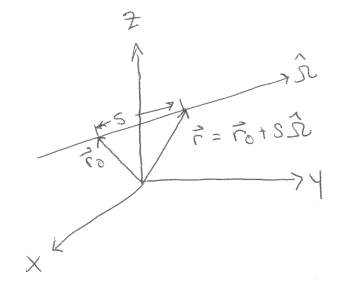
\includegraphics[keepaspectratio, width = 2.5 in]{../figs/moc-stream}    
    \end{center}
    \label{fig:stream}   
\end{figure}

Using this we can see
\[\frac{d\psi}{ds} = \frac{d\psi}{dx}\underbrace{\frac{dx}{ds}}_{\mu} + \frac{d\psi}{dy}\underbrace{\frac{dy}{ds}}_{\eta} + \frac{d\psi}{dz}\underbrace{\frac{dz}{ds}}_{\xi}\:,\]
which shows 
\[\frac{d\psi}{ds} = \vOmega \cdot \nabla \psi\:,\]
Now we can look at
\[\frac{d}{ds}\psi(\rvec_0 + \vOmega s, \vOmega, E) + \Sigma_t \psi = q(\rvec_0 + \vOmega s, \vOmega, E)\:.\]
This is a derivative along a characteristic curve. 
The equation is a linear, first-order ODE that can be integrated. 
We will do this by introducing an integrating factor: $\exp[\int^s ds'' \: \Sigma_t(\rvec_0 + \vOmega s'', E)]$. 

\end{document}
